\section{Cenni Matematici}
\subsection{L'operazione di convoluzione}
Nella sua forma più generale, la convoluzione è un'operazione di 
combinazione su due funzioni che restituisce una terza funzione.
Più formalmente, la convoluzione di due funzioni  $f(t)$ e $g(t)$, chiamate rispettivamente 
\textbf{funzione di input} e \textbf{kernel}, è definita come l'integrale del 
prodotto di $f(t)$ con una versione traslata e 
rovesciata di $g(t)$.  Formalmente può essere descritto come:
\begin{equation}
    (f*g)(t)=\int_{-\infty}^{+\infty}f(\tau)g(t-\tau)d\tau
\end{equation}
Il concetto di convoluzione qui può essere inteso come il "ribaltamento" 
della funzione $g(t)$, seguito dal "traslare" lungo la funzione $f(t)$, 
moltiplicando punto per punto, e integrando per ottenere la nuova funzione 
risultante \cite{Definizione_convoluzione_int,ALL_DEEP_LEARNING}.


\subsection{La convoluzione discreta}
In pratica, soprattutto in applicazioni digitali (come nelle reti neurali 
convoluzionali), si usa una versione discreta della convoluzione. 
Per due sequenze discrete $f(n)$ e $g(n)$, definite su $\mathbb{Z}$, 
la convoluzione discreta è definita come:
\begin{equation}
    S(n) = (f * g)(n) = \sum_{a\ =\ - \infty}^{\infty}{f(a)\cdot g(n - a)}
    \label{eq:convoluzioneDiscretaFormula}
\end{equation}
Questa formula è molto simile a quella della convoluzione continua, con la differenza 
che al posto dell'integrale abbiamo una somma discreta \cite{Definizione_convoluzione_int, ALL_DEEP_LEARNING}.

\subsection{La convoluzione nelle CNN}
Tuttavia, nelle reti convoluzionali, l’input è un array multidimensionale di dati mentre il 
kernel è un array multidimensionale di parametri che dipendono dall'algoritmo di learning scelto.

Entrambi questi array spesso sono chiamati \textbf{Tensori}. Riprendendo la formula \eqref{eq:convoluzioneDiscretaFormula}, la
sommatoria infinita potrà essere vista come una sommatoria su un numero finito di elementi 
di un array, su cui applicare la convoluzione in uno o più assi: ad esempio se
ricevessimo una immagine $I$ in 2D come input dovremmo usare un kernel in due dimensioni 
\cite{ALL_DEEP_LEARNING}.
Quindi la formula \eqref{eq:convoluzioneDiscretaFormula} può essere riscritta come:

\begin{equation}
    S(i,j)=(I*K)(i,j)=\sum_m \sum_n I(m,n)\cdot K(i-m,j-n)
    \label{eq:convoluzioneFormula1}
\end{equation}

Considerando anche la commutatività della convoluzione:

\begin{equation}
    S(i,j)=(I*K)(i,j)=\sum_m \sum_n I(i-m,j-n)\cdot K(m,n)
    \label{eq:convoluzioneFormula2}
\end{equation}



Talvolta, le equazioni \eqref{eq:convoluzioneFormula1} e \eqref{eq:convoluzioneFormula2} 
sono indicate in modo improprio come \textbf{ funzioni di correlazione (correlation functions)}.

\subsection{Cross-Correlation}
Nelle applicazioni pratiche, si usa spesso una variante semplificata della correlazione, 
chiamata \textbf{cross-correlation (correlazione incrociata)}.
La differenza principale risiede nel fatto che non si effettua 
l’inversione del kernel (flipping del kernel) \cite{ALL_DEEP_LEARNING}. 

La cross-correlation è descritta dalla seguente formula:
\begin{equation}
    S(i,j)=(I*K)(i,j)=\sum_m \sum_n I(i+m,j+n)\cdot K(m,n)
    \label{eq:Cross-Correlation}
\end{equation}

L'operazione di cross-correlation può essere visualizzato come:
\begin{figure}[h]
    \centering
    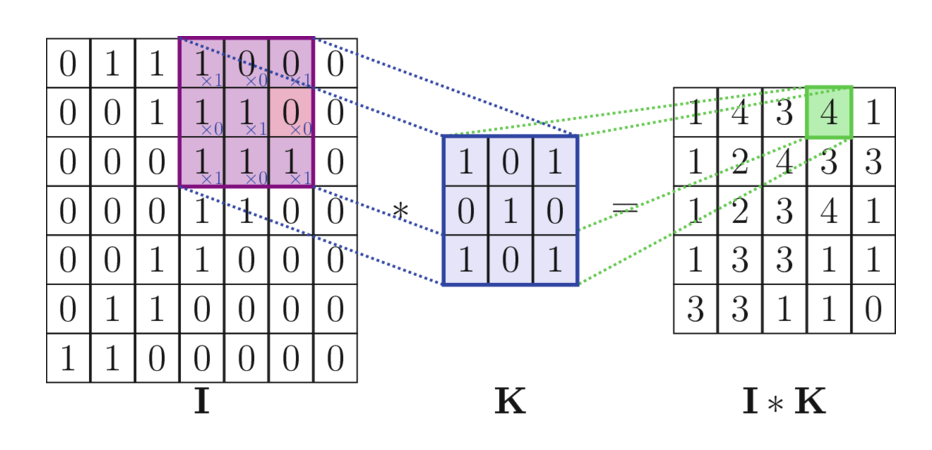
\includegraphics[width=0.8\textwidth]{Immagini/Grafici/convoluzione.png}
    \caption{Esempio di una convoluzione \cite{ELEMENTI_CNN_1,ALL_DEEP_LEARNING}.}
    \label{fig:convoluzione}
    %Figura 2.1: Esempio schematico di un neurone
\end{figure}

In alcuni casi, viene utilizzata una variante della formula \eqref{eq:Cross-Correlation}. Questa
formula si differisce soltanto dall'utilizzo di un bias, una costante che viene aggiunta al risultato 
finale della convoluzione. 
\begin{equation}
    S(i,j)=(I*K)(i,j)= b + \sum_m \sum_n I(i+m,j+n)\cdot K(m,n)
    \label{eq:Cross-Correlation_bias}
\end{equation}

\subsection{La convoluzione in tre dimensioni}
Un altro tipo di convoluzione che si utilizza spesso è la convoluzione 3D. 
Essa consiste nell'applicare un filtro a 3 dimensioni al set di dati.
Questo filtro si muove in 3 direzioni (x, y, z) per calcolare le 
rappresentazioni delle caratteristiche a basso livello \cite{ASPETTI_CONVOLUZIONE_1}.

\begin{figure}[H]
    \centering
    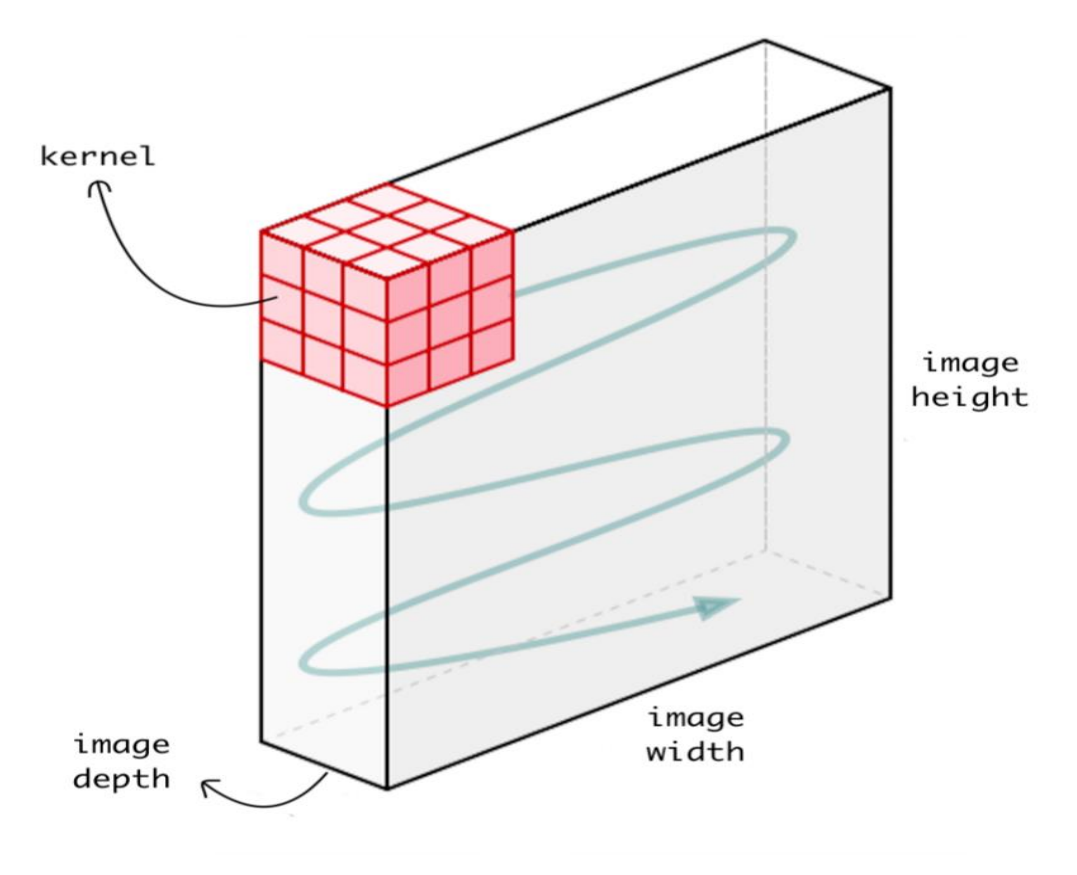
\includegraphics[width=0.45\textwidth]{Immagini/Generiche/3D_conv_moving.png}
    \caption{Rappresentazione convoluzione 3D \cite{MOVING_3D_Kernel}.}
    \label{fig:convoluzioneRGB}
\end{figure} 

Questa operazione può essere descritta come:

\begin{equation}
    S(i,j, k)=(I*K)(i,j,k)= b + \sum_m \sum_n \sum_p I(i+m,j+n, k+p)\cdot K(m, n, p)
    \label{eq:3D_conv_form}
\end{equation}

Questa tipologia di convoluzione è particolarmente utile per dati volumetrici 
come video, immagini mediche 3D, ecc.  La convoluzione 3D può essere applicata 
anche a input in spazio 2d, come le immagini. Oppure anche a sequenze di immagini,
come avviene nel telerilevamento, in cui si possono avere delle sequenze temporali 
di immagini \cite{ASPETTI_CONVOLUZIONE_1,MOVING_3D_Kernel}.

Quindi è una convoluzione particolarmente adatta per operare con dati che hanno 
un'estensione temporale o spaziale.

\begin{figure}[H]
    \centering
    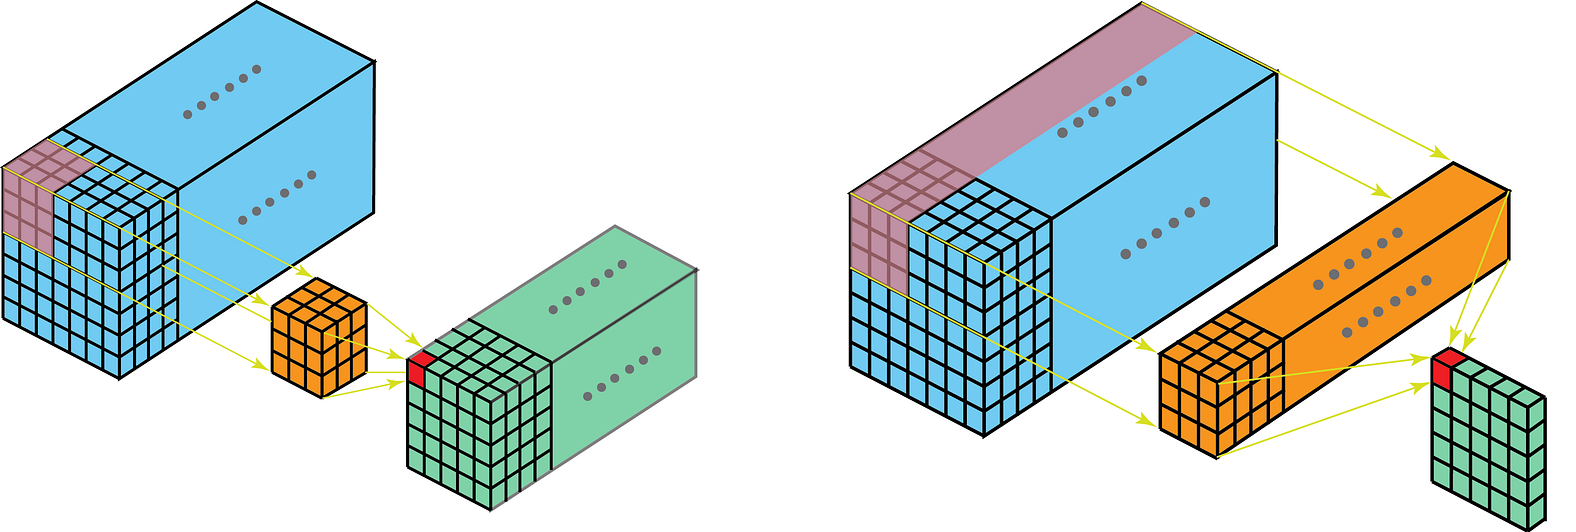
\includegraphics[width=0.8\textwidth]{Immagini/Generiche/Dimensione_kernel_con_3D.png}
    \caption{Dimensione delle feature map al variare del kernel \cite{Paragone_size_3D_kernel}.}
    \label{fig:size_3D_kernel}
\end{figure} 


\section{Aspetti e parametri della convoluzione}
\subsection{Convoluzione su più canali}
Nella pratica, la maggior parte delle immagini in ingresso ha 3 o più canali.
E questo numero aumenta quanto più ci si addentra in una rete. 

È qui che si rende utile una distinzione chiave tra i termini: mentre nel caso di 
1 canale i termini filtro e kernel sono intercambiabili, nel caso generale sono 
piuttosto diversi. Ogni filtro è in realtà un insieme di kernel, con un kernel 
per ogni singolo canale di ingresso allo strato e ogni kernel è unico.
Ogni filtro di uno strato di convoluzione produce un solo canale di uscita e lo fa 
in questo modo: Ciascuno dei kernel del filtro “scivola” sui rispettivi canali di 
ingresso, producendo una versione elaborata di ciascuno di essi.
Alcuni kernel possono avere pesi più forti di altri, per dare maggiore enfasi a 
determinati canali di ingresso rispetto ad altri 
(ad esempio, un filtro può avere un kernel del canale rosso con pesi più forti di 
altri, e quindi rispondere maggiormente alle differenze nelle caratteristiche del 
canale rosso rispetto agli altri).
Tutti i canali elaborati vengono poi sommati insieme al bias per formare il valore 
del canale in uscita \cite{ASPETTI_CONVOLUZIONE_2,ELEMENTI_CNN_1}.





% Quando l'input ha più di un canale ($C_{in} > 1$), ogni canale dell'output viene calcolato 
% combinando i valori convoluzionati di tutti i canali dell'input, come mostrato nella 
% somma \`a doppio indice $\sum_{k=0}^{C_{in}-1}$. In altre parole, il \textit{C-out}-esimo 
% canale dell'output \`e il risultato della somma ponderata (tramite i filtri $\text{weight}$) 
% di tutti i canali dell'input.

% Ad esempio, per un input con $C_{in}=3$ (immagini RGB), ciascun filtro 
% $\text{weight}(C_{out}, k)$ viene applicato rispettivamente ai tre canali $R$, $G$, e $B$ 
% dell'input. I risultati vengono sommati elemento per elemento e combinati con il bias per 
% produrre l'output del \textit{C-out}-esimo canale.
% Questa operazione può essere visualizzato come:
\begin{figure}[H]
    \centering
    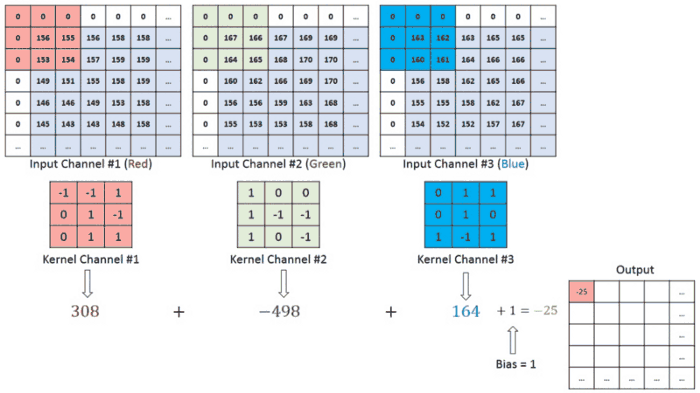
\includegraphics[width=0.95\textwidth]{Immagini/Generiche/convoluzione_canali.png}
    \caption{Illustrazione dell'operazione di convoluzione su più canali 
    \cite{ELEMENTI_CNN_1}.}
    \label{fig:convoluzioneRGB}
\end{figure}

Come possiamo osservare dalla figura (\ref{fig:convoluzioneRGB}), questa operazione 
è molto simile alla convoluzione 3D. Infatti, in alcuni casi è possibile anche 
utilizzare la convoluzione 3D definendo la profondità come il numero 
dei canali dell'immagine.
Tuttavia, nelle sequenze di immagini, si hanno più immagini composte da più canali.
In questo caso si esegue la stessa operazione dalla figura (\ref{fig:convoluzioneRGB}):
si utilizza un kernel 3D per ogni canale ma che opera su tutta la sequenza.

\subsection{Parametri della convoluzione}
In Pytorch il comportamento della convoluzione è regolato principalmente dai seguenti 
parametri \cite{CONV_PYTORCH}:

\begin{itemize}
    \item \textbf{Kernel size}: Questo parametro determina la dimensione del kernel. 
    In genere vengono utilizzati kernel di dimensioni ridotte, preferibilmente 
    valori dispari come: 1x1, 3x3, 5x5 e 7x7. 
    In alcune applicazioni, capita anche di utilizzare kernel più grandi, come 11x11.
    
    \item \textbf{Stride}: Lo stride \`e il numero di pixel con cui si fa scorrere la matrice 
    dei filtri sulla matrice di input. Quando lo stride \`e 1, i filtri vengono spostati di un 
    pixel alla volta. Quando lo stride \`e 2, i filtri saltano di 2 pixel alla volta mentre 
    vengono fatti scorrere. Uno stride maggiore produce mappe di caratteristiche pi\`u piccole.

    \item \textbf{Padding}: A volte \`e conveniente espandere la matrice di input (l'immagine) con degli 
    zeri intorno al bordo, in modo da poter applicare il filtro agli elementi confinanti 
    della matrice dell'immagine di input. Una caratteristica interessante del padding a 
    zero \`e che ci permette di controllare la dimensione delle mappe di caratteristiche. 
    L'aggiunta di zero padding \`e chiamata anche convoluzione ampia, mentre l'assenza di zero 
    padding sarebbe una convoluzione stretta. 
    Il valore da utilizzare come padding \`e arbitrario ma tipicamente si utilizza il valore 0.

    \item \textbf{Numero di filtri / canali in uscita}: Questo parametro corrisponde al numero di 
    filtri utilizzati per l'operazione di convoluzione. Ogni filtro viene utilizzato per creare un
    nuovo canale sull'immagine di uscita. Tutti questi canali corrispondono alle feature map.

    % \item \textbf{Bias}: Questo parametro booleano viene utilizzato per specificare se utilizzare
    % il bias nella convoluzione.

    \item \textbf{Dilatation}: Questo parametro viene utilizzato per controllare la spaziatura tra i 
    punti del kernel.

    \begin{figure}[H]
        \centering
        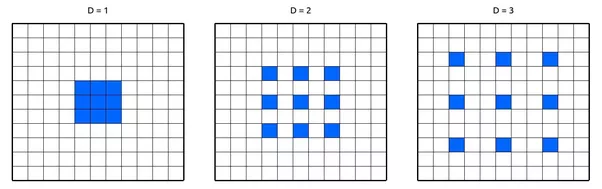
\includegraphics[width=0.9\textwidth]{Immagini/Generiche/dilatation_conv.png}
        \caption{Rappresentazione della Dilatation \cite{ASPETTI_CONVOLUZIONE_1}.}
        \label{fig:Dilatation}
    \end{figure}

\end{itemize}






%\subsection{Equivalenza tra la convoluzione 2D e 3D}


% \subsection{Come determinare le dimensioni della feature map}
% La dimensione dell'uscita dello strato convoluto è determinata da diversi fattori, 
% tra cui la dimensione dell'ingresso, la dimensione del kernel, lo stride e il padding. 
% Per calcolare l'altezza ($H$) e la larghezza ($W$) della feature map si utilizzano le 
% seguenti formule:

% \begin{equation}
%     H_{out}=1+\frac{H_{in} + 2\cdot \text{padding} - \text{Kernel}_{\text{height}}}{\text{stride}}
% \end{equation}

% \begin{equation}
%     W_{out}=1+\frac{W_{in} + 2\cdot \text{padding} - \text{Kernel}_{\text{width}}}{\text{stride}}
% \end{equation}

% \section{La convoluzione di Pytorch}
% In Pytorch, la convoluzione \`e definita nel seguente modo:
% \begin{equation}
%     \text{out}(N_i, C_{out_j}) = \text{bias}(C_{out_j}) + \sum_{k=0}^{C_{in}-1} \text{weight}(C_{out_j}, k) * \text{input}(N_i, k)
% \end{equation}
% In cui:
% \begin{itemize}
%     \item $C_{in}$: \`E il numero totale dei canali nell'input.
%     \item $C_{out_j}$: \`E il $j$-esimo canale di uscita.
%     \item $N_i$: Corrisponde all'elemento $i$-esimo del batch
%     % \item $\text{out}(N_i, C_{out})$: \`E il valore dell'output della convoluzione per la \textit{i-esima} immagine del batch $N_i$ e il \textit{C-out}-esimo canale dell'output.
%     % \item $\text{bias}(C_{out})$: \`E un termine scalare che viene aggiunto a ciascun valore calcolato per il canale $C_{out}$, se il bias \`e abilitato (\texttt{bias=True}).
%     % \item $\text{weight}(C_{out}, k)$: \`E il filtro di convoluzione (o kernel) associato al \textit{C-out}-esimo canale dell'output e al \textit{k-esimo} canale dell'input. \`E un tensore di dimensioni $\text{kernel\_size} \times \text{kernel\_size}$.
%     % \item $\text{input}(N_i, k)$: \`E il valore dell'input per la \textit{i-esima} immagine del batch $N_i$ e il \textit{k-esimo} canale dell'input.
% \end{itemize}
% Come si può osservare, Pytorch modifica la formula della Cross-Correlation \eqref{eq:Cross-Correlation} 
% aggiungendo un bias e facendo la summatoria delle convoluzioni svolte su ogni canale dell'immagine (o feature map) di input.

